%% ===========================================================================
\FloatBarrier
\section{Numerical results and discussion}
\label{sec:results}
%% ===========================================================================

The five design questions raised in Sec.~\ref{sec:intro} are answered here, one
subsection each: whether the direction in which the microstructure is sampled
matters, what the size and the shape of the window do, whether thinning a device
helps, what the memory order and the relaxation time do to the damping, and what
the four electrode configurations return for one strip. Every number quoted is a
solved eigenvalue or a time march of the model of Sec.~\ref{sec:formulation},
discretized as in Sec.~\ref{sec:fem} and checked as in
Sec.~\ref{sec:verification}. The inputs are those of Sec.~\ref{sec:formulation}; the worked calculation
is in Sec.~\ref{sec:worked} and the tables in \ref{app:data} and
\ref{app:verification}.

\FloatBarrier
\subsection{Window orientation and window aspect ratio}
\label{sec:orientation}

Figure~\ref{fig:orientation} shows what the orientation of an anisotropic
sampling window is worth, which is the first design question because the
gradient energy is linear in the second-moment tensor $M$ and a rotation of the
window changes $M$ without changing the strip. The window is held at a
half-width of \SI{3}{\micro\meter} along its long axis; its aspect ratio is
${\rm AR}=a_1/a_2$. The strip is
\SI{200}{\micro\meter}$\times$\SI{10}{\micro\meter}, for the poling-$x$
configuration that carries the response; physically, the window is the domain
over which the microstructure of the film is averaged, so its orientation
decides which component of the strain gradient the material is asked to
transmit. Over the $6\times19$ cuboid cases the extensional mode remains the one
with the largest coupling, its short-circuit frequency varying smoothly from
$4907$ to \SI{5296}{kHz}, so the mode identity is not in question while the
window turns.

\subsubsection{Why one quadrant is computed}

The strip maps onto itself under $\theta\to\theta+180^\circ$. The second
invariance is a symmetry of the whole problem and not of the energy alone: the
gradient energy is \emph{linear} in $M$, so a change of sign of $M_{12}$ by
itself changes the response, and what leaves it unchanged is the reflection
$y\to-y$, which maps $\theta\to-\theta$ and at the same time maps the strip,
the electrode pair and -- for poling along $x$, the configuration plotted here
-- the material onto themselves. The response is therefore even in $\theta$ for
the poling-$x$ configuration; for poling along $y$ the same reflection reverses
the poling direction and is not a symmetry of the material, so only the period
$180^\circ$ holds and the orientation study is confined to poling $x$. Neither
invariance is assumed: both are evaluated at \SI{15}{\degree} intervals for the
extreme aspect ratios, where they reproduce the computed points to
$3\times10^{-11}$ relative.

\subsubsection{What the orientation is worth}

The extensional frequency and coupling move monotonically with $\theta$ and saturate by
$\theta=90^\circ$. The extensional frequency rises from $5012$ to
\SI{5296}{kHz} at ${\rm AR}=2$ and from $4907$ to \SI{5288}{kHz} at
${\rm AR}=10$, that is by $6$--$8\,\%$, while the coupling falls from $0.4448$
to $0.3786$ and from $0.4677$ to $0.3801$ between the same two orientations, a
change of $15$--$19\,\%$. The fundamental mode of the same strip, which carries
a coupling three orders of magnitude smaller, moves from \SI{146.4}{kHz} to
\SI{158.1}{kHz} at ${\rm AR}=10$. At $\theta=0^\circ$ the window aspect ratio is
worth $0.4448\to0.4677$ between ${\rm AR}=2$ and ${\rm AR}=10$, about
$5\,\%$, and the aspect ratios collapse onto $0.3786$--$0.3801$ at
$\theta=90^\circ$: once the long axis of the window is transverse to the strain
gradient, its aspect ratio no longer matters.

The coupling plotted here is the \emph{total} coupling of the extensional mode
and it is piezoelectric in the main; the flexoelectric contribution at
$\mu=10^{-6}$\,\si{\coulomb\per\meter} is of order $10^{-4}$
(Sec.~\ref{sec:thickness}), so the window acts on the modal coupling through
the gradient stiffness rather than by adding a flexoelectric term directly.
Figure~\ref{fig:design} separates the two. Panel (a) is the change of the
coupling against the aligned window: largest for the most elongated window,
$-18.7\,\%$ at ${\rm AR}=10$ and $\theta=90^\circ$, and weakest for the
squarest, $-14.9\,\%$ at ${\rm AR}=2$. Panel (b) is
$(M_{11}-M_{22})/(M_{11}+M_{22})$, shown for ${\rm AR}=2$, which
passes through zero at $45^\circ$ and changes fastest there. The coupling
follows the anisotropy of the second-moment tensor and not the shape of the
window. Hence the orientation of the window is a design variable worth
$15$--$19\,\%$ of the coupling, while the aspect ratio of an already elongated
window is worth $5\,\%$ or less once the window is turned transverse to the
gradient.

\begin{figure}[!htbp]
\centering
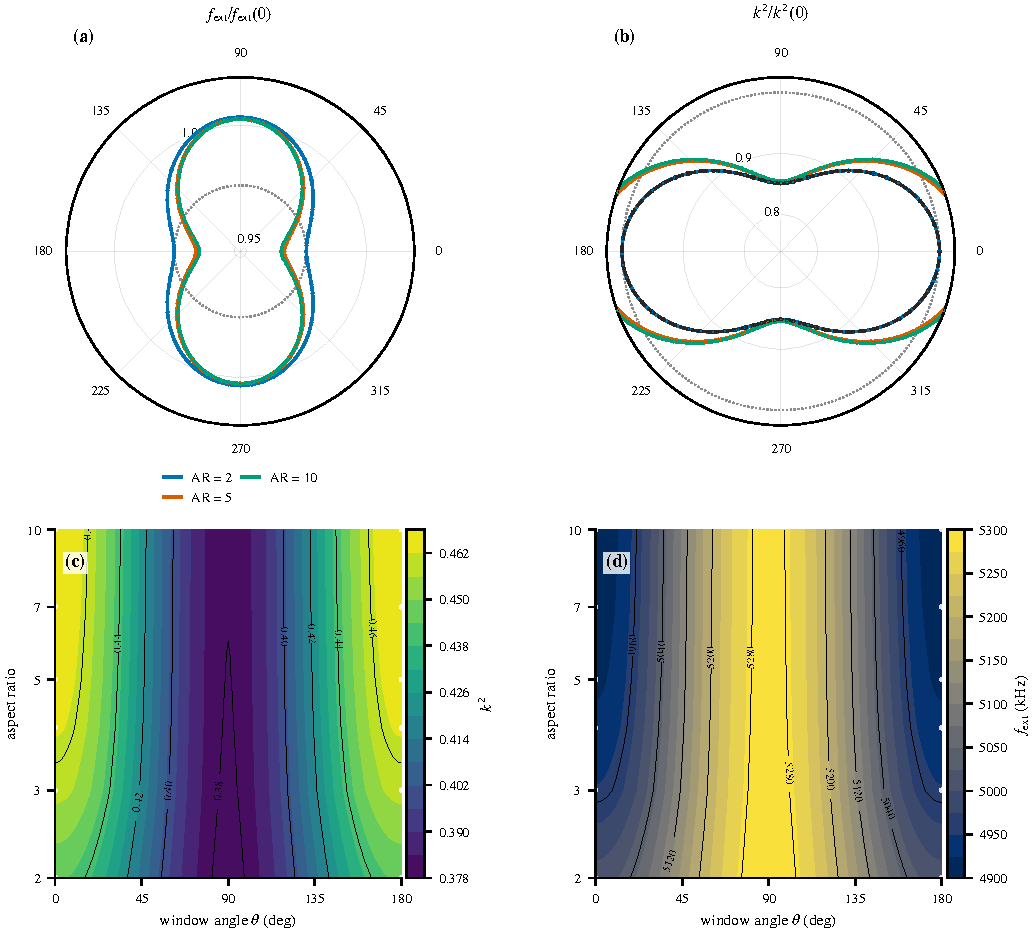
\includegraphics[width=\textwidth]{F4_orientation.pdf}
\caption{Variations of (a) the extensional frequency and (b) its coupling factor, both normalized to the aligned ${\rm AR}=2$ window, over the full circle of window orientation, and of (c) the coupling factor and (d) the frequency as maps over orientation and window aspect ratio, for a \SI{200}{\micro\meter}$\times$\SI{10}{\micro\meter} strip with poling along $x$, plane stress and a $24\times2$ mesh. Markers are computed points, lines a periodic spline. The long window half-width is \SI{3}{\micro\meter}.}
\label{fig:orientation}
\end{figure}

\begin{figure}[!htbp]
\centering
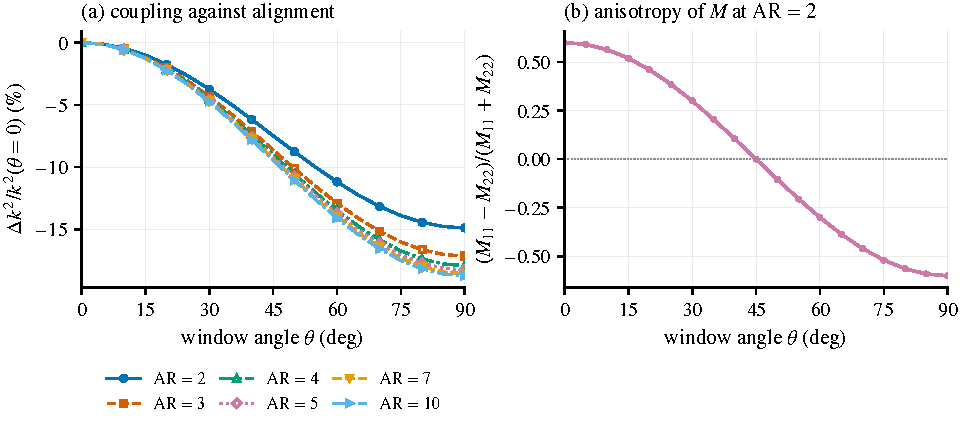
\includegraphics[width=0.86\textwidth]{F5_design.pdf}
\caption{Variations of (a) the change of the extensional coupling relative to the aligned window, one curve per window aspect ratio, and of (b) the anisotropy of the second-moment tensor at ${\rm AR}=2$, for the window and poling of Fig.~\ref{fig:orientation}. The coupling spans $4$ percentage points at $90^\circ$ and reaches $-18.7\,\%$ where the anisotropy of (b) is largest.}
\label{fig:design}
\end{figure}

\FloatBarrier
\subsection{Memory order, relaxation time and the damping map}
\label{sec:memorystudy}

Figure~\ref{fig:damping} shows how the two parameters of the dielectric law move
the damping of a mode, and the answer separates into a modeling and an
implementation question. The modeling question is the fractional
Kelvin--Voigt element of \eqref{eq:kv}, which differs measurably from the
integer-order element that finite element codes usually provide; physically,
$\alpha$ measures how broad the relaxation spectrum is, a single time constant
at $\alpha=1$ and a spectrum spread over decades below it, while $\tau$ is the
center of that spectrum and fixes the $\omega\tau$ at which the loss peaks. The
implementation question is the convolution of \eqref{eq:step}, which may
multiply the fully condensed stiffness $K_{\rm eff}$ or only the short-circuit
matrix $K_{uu}$; the two give different damping, and the difference is not a
numerical detail. The loss tangent \eqref{eq:tandelta} and its small-loss limit
\eqref{eq:zetasmall} of Sec.~\ref{sec:calib_alpha_tau} are what the map plots,
and the integer-order limit it is compared against is \eqref{eq:limitKV}.

\subsubsection{Which matrix carries the memory}

Table~\ref{tab:memory} reports the ring-down of the extensional mode (mode 4,
\SI{6.727}{MHz}) at $\tau=\SI{7.0974}{\nano\second}$, that is $\omega\tau=0.3$,
with an initial tip displacement that produces \SI{139.07}{\volt} of
open-circuit voltage at $t=0$. Three coupling numbers for that mode appear in
the paper and they come from two quantities:
$k^2_{4}(K_{uu})=0.4650$ is the mode-based measure on the elastic memory matrix
$K_{uu}$ and $k^2_{4}(K_{sc})=0.4583$ is the same measure on the short-circuit
stiffness $K_{sc}$, both on the $24\times2$ mesh of the ring-down; the third,
$0.4580$ in Sec.~\ref{sec:application}, is $k^2_{4}(K_{sc})$ again,
recomputed with $\mu=0$ because that section quotes the material without
flexoelectricity. The gap of $1.5\,\%$ between $0.4650$ and $0.4583$ reflects the
choice of short-circuit stiffness in the coupling measure, while the
$0.07\,\%$ between $0.4583$ and $0.4580$ reflects the inclusion of $\mu$.

The damping ratio is extracted from two successive peaks with
\eqref{eq:zeta}. At the $\omega\tau=0.3$ of Table~\ref{tab:memory} the ratio of
two successive voltage peaks is $2.5947$, so $\delta=0.95345$ and
$\zeta_{\rm eff}=0.15003$ for $K_{\rm eff}$ at $\alpha=1$, against the exact
$\omega\tau/2=0.15000$: the implementation reproduces the classical limit to
$0.02\,\%$. Refining the step gives $\zeta_{\rm eff}=0.150111$, $0.150057$ and
$0.150029$ at $N$, $2N$ and $4N$ steps over twenty periods, so the residual is
first order in $\Delta t$ (observed order $0.97$) and extrapolates to
$0.150000$; every ring-down quoted in this section is run at the $4N$ step.
Replacing $K_{\rm eff}$ by $K_{uu}$ removes the piezoelectric contribution from
the memory and takes the ratio $\zeta(K_{uu})/\zeta(K_{\rm eff})$ at $\alpha=1$
down to $0.450$, so the short-circuit memory dissipates $55\,\%$ less. The
difference is of the order of the coupling ($k^2_{4}=0.4650$) but does
\emph{not} reduce to the naive factor $1-k^2=0.535$: the two memories differ by
the piezoelectric stiffness that the condensation puts into $K_{\rm eff}$, and
its effect on the ring-down has to be computed rather than estimated. For a
strongly piezoelectric device the distinction belongs in the model statement,
not in the implementation.

Neither matrix is derived from a dielectric relaxation; both are placements of
the fractional element inside a condensed model. One law can be derived
exactly. If the permittivity itself relaxes,
$D_k=e_{kij}\varepsilon_{ij}+\kappa_{kl}[1+(\tau\partial_t)^{\alpha}]E_l$,
then $\nabla\cdot\bm D=0$ carries the Caputo derivative of the field, and
condensing the potential moves the memory onto the piezoelectric stiffening
$B_iC^{-1}B_i^{\mathsf T}$, that is onto exactly the part of $K_{\rm eff}$ that
the condensation adds over $K_{uu}$. That is a third possibility, bracketed by
the two matrices tabulated: $K_{\rm eff}$ remembers the whole condensed
stiffness and $K_{uu}$ none of it. The ratio $0.450$ belongs to the
$\alpha=1$ row of Table~\ref{tab:memory} and to this device.

%% The memory-matrix comparison, moved from the appendix to the text.
\begin{table}[!htbp]
\centering
\small
\caption{Ring-down with the memory carried on the condensed stiffness
$K_{\rm eff}$ and on the short-circuit stiffness $K_{uu}$ (mode 4,
\SI{6.727}{MHz}, $\omega\tau=0.3$). At $\alpha=1$ the entry is the damping
ratio \eqref{eq:zeta}; at $\alpha=0.7$ the decay is not exponential and the
entry is the first-period decrement.}
\label{tab:memory}
\begin{tabular}{@{}lcc@{}}
\toprule
memory matrix & $\alpha=1$: $\zeta_{\rm eff}$ &
  $\alpha=0.7$: first-period $\zeta$ \\
\midrule
$K_{\rm eff}$ & $0.15003$ & $0.1942$ \\
$K_{uu}$      & $0.06746$ & $0.0831$ \\
\midrule
ratio $K_{uu}/K_{\rm eff}$ & $0.450$ & $0.428$ \\
\bottomrule
\end{tabular}
\end{table}


\subsubsection{Decay at fractional order}

At $\alpha=0.7$ the free decay is not exponential and a single damping ratio
does not exist: the successive decrements of the $K_{\rm eff}$ ring-down are
$1.244$, $1.547$, $0.010$, $0.403$, $0.240$ and $0.151$; the first, second,
fourth, fifth and sixth of them are unchanged to three digits between
$\Delta t$, $\Delta t/2$ and $\Delta t/4$, so they are a property of the
fractional element -- whose relaxation is a Mittag-Leffler function, not an
exponential -- and not of the step, while the third is a near-cancellation
between two peaks of comparable height. A straight line fitted to $\ln A_k$, with $A_k$ the successive peak amplitudes,
over the twenty periods therefore returns a number that is not a damping ratio,
which is why the $\alpha=0.7$ column of Table~\ref{tab:memory} carries the
first-period decrement rather than a fitted slope. The $\alpha=1$ entries are
unaffected: there the twenty successive decrements agree to $7\times10^{-10}$
relative, which is why \eqref{eq:zeta} applies.

\subsubsection{Fractional against integer-order element}

The fractional element differs from the integer-order one by more than
accuracy; it differs in shape. At the device point $\omega\tau=0.3$ the
Kelvin--Voigt model over-predicts the modulus by $3.5\,\%$ at $\alpha=1$ and by
$22.6\,\%$ at $\alpha=0.7$; at $\omega\tau=1$ the ratio of the two is $1.35$
and $1.62$, and at $\omega\tau=100$ the integer-order model is wrong by a
factor $91$. A single-relaxation fit is unusable outside the narrow band where
it was fitted, which is the band a design map is meant to cover.

\subsubsection{The damping map}

Figure~\ref{fig:damping}(a) is the pole of \eqref{eq:kvfreq} in the complex
plane, traced over $\omega\tau$ for seven relaxation times and colored by
$\tau$, with markers at five Caputo orders; Fig.~\ref{fig:damping}(b) is the
damping ratio $\zeta=-\mathrm{Re}\,s/|s|$, where $s$ is the dimensional
complex pole and $\omega_0$ the undamped angular frequency, over the
$(\alpha,\omega\tau)$ plane. Both are computed with branch continuation: the
root is followed from one $\omega\tau$ to the next by initializing the Newton
iteration at the adjacent converged pole, without which the iteration jumps to a spurious
root of the negative-real-part branch. All poles lie in the left half-plane for
every $(\alpha,\tau)$ examined, so the fractional Kelvin--Voigt element is
dissipative by construction. The integer-order case sits at
$|\mathrm{Im}\,s|/\omega_0\simeq1$ for $\omega\tau\lesssim0.1$ and moves down
and to the right as $\omega\tau$ grows, so the dashpot lowers the frequency and
eventually over-damps the mode: at $\omega\tau=10$ the imaginary part has
vanished and $\zeta=1$. The fractional cases fan \emph{upward}: a spring-pot
with $\alpha<1$ raises the damped frequency as $\tau$ grows, because the
fractional modulus grows sub-linearly rather than linearly in $\omega$. At
$\omega\tau=10$ and $\alpha=0.5$ the damped frequency is $2.13\,\omega_0$
($2.45\,\omega_0$ at $\alpha=0.7$), against $\mathrm{Im}\,s=0$ for $\alpha=1$ at
the same $\omega\tau$. The ratio in Fig.~\ref{fig:damping}(b) increases with
both $\alpha$ and $\omega\tau$ and reaches $\zeta\to1$ for $\alpha\to1$ and
large $\omega\tau$; for small $\alpha$ it is flat, because a spring-pot with a
broad relaxation spectrum produces a damping that depends only weakly on the
device frequency. That flatness is the qualitative reason the fractional
description is used for dielectric loss in the first place. The band
$\omega\tau\le1$, which contains the strip mode at \SI{6.73}{MHz} for every
$\tau\le\SI{32}{\nano\second}$ used here, is the one in which the element is
calibrated and claimed. Hence, in the range where the element is used, $\alpha$
sets the shape of the decay and $\tau$ sets where the loss peaks, and neither of
them alone fixes a damping ratio.

\begin{figure}[!htbp]
\centering
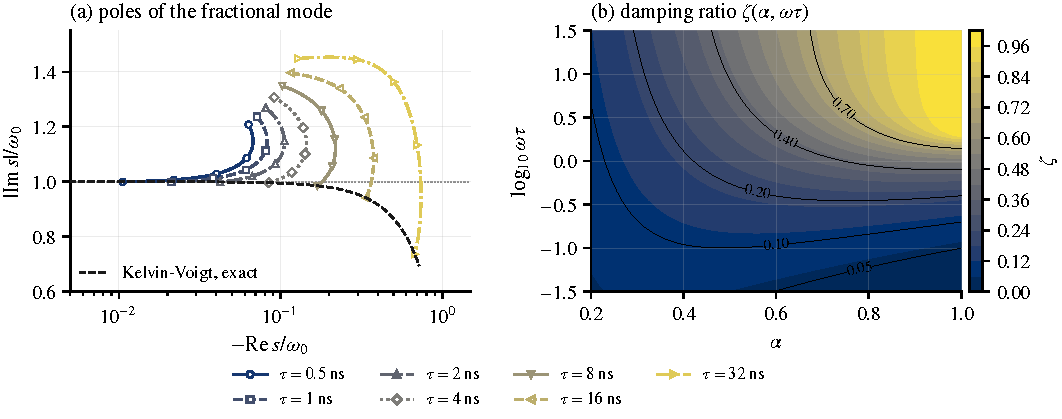
\includegraphics[width=\textwidth]{F6_damping.pdf}
\caption{Variations of (a) the pole of a mode at $f_0=\SI{6.73}{MHz}$ ($\omega_0=2\pi f_0$) over $\omega\tau=0.02$--$1.35$ for seven relaxation times, identified by $\tau$ in the legend and distinguished by line style and marker, with markers at five Caputo orders, and of (b) the damping ratio over $\omega\tau=10^{-1.5}$--$10^{1.5}$ and $\alpha=0.2$--$1$ with labeled contours, for the fractional Kelvin--Voigt element with branch continuation. The dashed arc is the exact Kelvin--Voigt locus, on which every $\alpha=1$ pole lies. Fractional poles fan upward, integer-order poles over-damp.}
\label{fig:damping}
\end{figure}

\FloatBarrier
\subsection{Window size and shape against the second moment}
\label{sec:windowshape}

Figure~\ref{fig:window} shows what the size and the shape of the window do on
a problem whose classical answer is known, which is the second design question
because the strain-gradient energy is linear in $M$: if that linearity holds,
the shape cannot matter once $M$ is fixed, and any size dependence must enter
through $M$ alone. Panel~(a) is the numerical statement of
Sec.~\ref{sec:window} on an isotropic plane-strain test problem (rectangle
$1\times0.2$, $20\times4$ mesh, uniaxial edge traction, displacement averaged
over the loaded edge), plotted against the normalized window size for an
ellipsoidal window of semi-axis $l$, a cuboidal window of half-width $l$, and a
cuboidal window scaled to carry the same $M$ as the ellipsoid,
$a=l\sqrt{3/5}$. The third curve is indistinguishable from the first: within
the adopted second-moment model the shape of the window is irrelevant at fixed
$M$. The second curve shows the error made by ignoring the distinction: equal
half-widths instead of equal $M$ over-stiffen the response, and the
discrepancy grows with the window size. Writing $L_x$ for the rectangle length, at $l/L_x=0.2$ a cuboid of half-width
$l$ retains $0.922$ of the classical loaded-edge displacement, an ellipsoid of
semi-axis $l$ retains $0.941$, and the equal-$M$ cuboid sits on the ellipsoid
curve to the third decimal. At fixed $M$ the shape of the window is therefore
immaterial to $10^{-3}$, which is the coefficient ratio $5/3$ in the gradient
stiffness seen from the response side. The assumed operating range is
$a/L\le0.2$, the right-hand edge of the figure.

Panels (b) and (c) are the corresponding static statement. The clamped strip of
Table~\ref{tab:params} is solved under an end load for three window sizes and
each solution is compared with the classical one of the same geometry and load.
The gradient terms stiffen the member. The difference against the classical
solution vanishes at the clamped edge, where both fields satisfy the same
kinematic conditions, and then accumulates along the member instead of decaying
over a thin layer: at these window sizes the gradient effect is distributed
rather than local, and its size grows with the window. That is why $a/L\le0.2$
is quoted as an assumed operating range and not as a validated truncation
threshold. Hence, at a fixed second moment the shape of the window is immaterial
to the third decimal, and its size and its anisotropy are the only window
parameters left in the model. The entries of \ref{app:Mcoeff} used here are the
ellipsoidal second moment \eqref{eq:Mellip} and its rotation \eqref{eq:Mrot}, and
the classical profile follows from \eqref{eq:limitM} with flexoelectricity
suppressed.

\begin{figure}[!htbp]
\centering
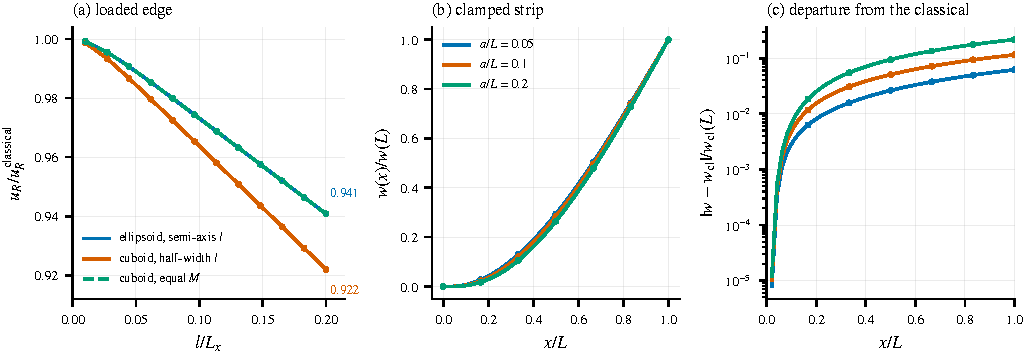
\includegraphics[width=\textwidth]{F7_window.pdf}
\caption{Variations of (a) the loaded-edge displacement of an isotropic plane-strain rectangle against normalized window size, for an ellipsoid, a cuboid of equal half-width and a cuboid of equal second moment, and of (b) the deflected shape of a clamped strip for three window sizes together with (c) its difference from the classical profile. Windows of equal second moment collapse onto one curve. Panel (a) uses a $1\times0.2$ rectangle and a $20\times4$ mesh under uniaxial edge traction; panels (b,c) use Table~\ref{tab:params} with $a/L=0.05$, $0.1$ and $0.2$.}
\label{fig:window}
\end{figure}

\FloatBarrier
\subsection{Thickness: a flexoelectric size effect against a thickness-independent
piezoelectric coupling}
\label{sec:thickness}

Figure~\ref{fig:thickness} shows whether thinning a device helps, which is the
third design question because the two available couplings scale differently
with thickness: physically, a bending mode of thickness $h$ carries a strain
gradient of order $\kappa_c/h$, so a coupling proportional to the gradient
grows as $h^{-2}$, while a coupling proportional to the strain does not grow
at all. The figure answers the question by solving the same strip at eight
thicknesses between \SI{10}{\micro\meter} and \SI{1}{\micro\meter} with a
\SI{200}{\micro\meter} length and the window held at half-widths
$3\times1$\,\si{\micro\meter}, so that the thickness is the only variable;
Table~\ref{tab:thickness} lists the sweep, and \ref{app:verification} carries
the mesh witnesses. One qualification belongs to the two thinnest points: the
window half-thickness is \SI{1}{\micro\meter} throughout, so at
$h=\SI{2}{\micro\meter}$ it is half the strip and at $h=\SI{1}{\micro\meter}$
it equals the strip. The second-moment tensor of the full window is used at
every thickness and no truncated-window boundary correction is applied, so $M$
acts there as a local effective gradient tensor rather than as the moment of a
window small compared with the body. The two panels are two electrical
configurations of that strip: panel~(a) is poled through the thickness
(electrodes on the long faces, gap $h$, $\kappa_{yy}=\kappa_{33}$) and
panel~(b) along the length (electrodes on the short faces, gap $L$,
$\kappa_{xx}=\kappa_{33}$).

\begin{figure}[!htbp]
\centering
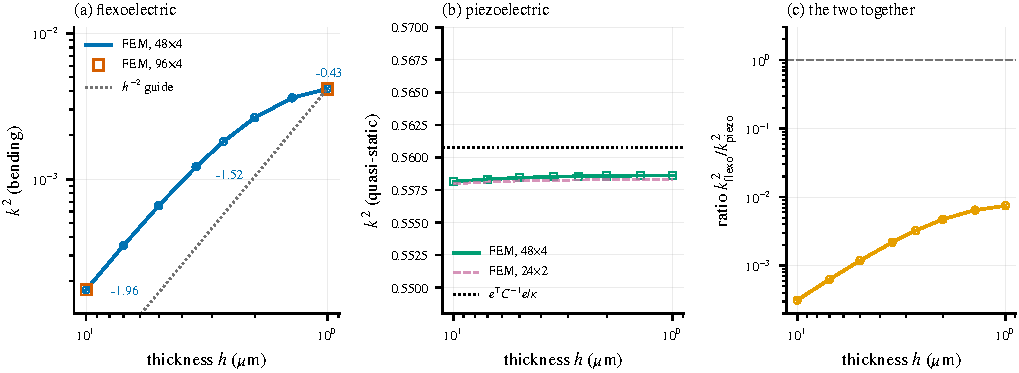
\includegraphics[width=\textwidth]{F8_thickness.pdf}
\caption{Variations of (a) the flexoelectric bending coupling against strip thickness at eight thicknesses, with local log--log slopes, a $96\times4$ witness at both ends and the $h^{-2}$ guide, of (b) the piezoelectric extensional coupling of the same strip with $\mu=0$, constant to $0.09\,\%$ over $10\to1\,\si{\micro\meter}$, and of (c) their ratio, which spans $3.1\times10^{-4}$ to $7.5\times10^{-3}$.}
\label{fig:thickness}
\end{figure}

\subsubsection{The flexoelectric size effect}

The flexoelectric coupling rises by a factor $24$ from $1.74\times10^{-4}$ at
\SI{10}{\micro\meter} to $4.2\times10^{-3}$ at \SI{1}{\micro\meter}. Its local
log--log slope is $-1.96$ at the thick end, close to the $h^{-2}$ scaling of a
gradient effect with a window much smaller than the thickness, and falls to
$-1.52$, $-1.26$ and $-0.43$ on the successively thinner pairs, the seven
segments spanning $-1.96$ to $-0.43$. The saturation survives refinement: a
$96\times4$ witness reproduces the $48\times4$ values to $0.04\,\%$ and
$0.35\,\%$ at the two ends of the range, and the residual at $\mu=0$ is
$1.0\times10^{-10}$, seven orders of magnitude below the signal. The
dimensionless group that explains the saturation is $a_2/h$, the window
half-thickness over the strip thickness, which runs from $0.10$ at
$h=\SI{10}{\micro\meter}$ to $1.0$ at \SI{1}{\micro\meter}: the slope decreases
monotonically as $a_2/h$ grows, which is what a fixed-size window does when it
smears a through-thickness gradient that becomes comparable to the strip. The
same stiffening appears in the fundamental frequency, which follows
$210.4,108.0,50.2,34.7$\,kHz where pure Euler--Bernoulli scaling from the
thickest strip would give $210,105,42,21$\,kHz.

Figure~\ref{fig:modetrack} records the mode identification behind the sweep,
which is what makes the factor $24$ a statement about one mode. The mode shape
at each thickness is compared with the one at $h=\SI{10}{\micro\meter}$ through
the modal assurance criterion, which stays above $0.999$ across the whole
sweep, and the ratio $f_2/f_1$ stays between $6.21$ and $6.27$: the branch that
carries the coupling is separated from its neighbors by the same margin at
every thickness.

\begin{figure}[!htbp]
\centering
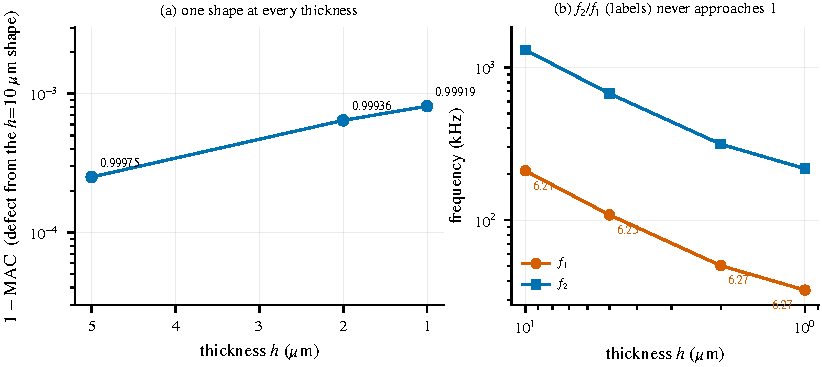
\includegraphics[width=0.90\textwidth]{FB1_tracking.pdf}
\caption{Variations of (a) the defect $1-\mathrm{MAC}$, the MAC being the modal assurance criterion, between the mode shape at each thickness and the shape at $h=\SI{10}{\micro\meter}$, with the MAC printed, and of (b) the frequencies of the first two modes and their ratio, over a sweep from $10$ to $1\,\si{\micro\meter}$. The tracked branch stays within $10^{-3}$ of itself, so the identification is unambiguous. Inputs match Fig.~\ref{fig:thickness}(a).}
\label{fig:modetrack}
\end{figure}

Figure~\ref{fig:modes} complements this one-mode identification with the
spatial structure of the tracked branch. The surface is the computed
open-circuit bending displacement, colored by the solved electric potential,
and the inset gives a labeled two-dimensional reading of the same potential on
the strip coordinates so that the through-thickness variation is not inferred
from the three-dimensional projection alone.

\begin{figure}[!htbp]
\centering
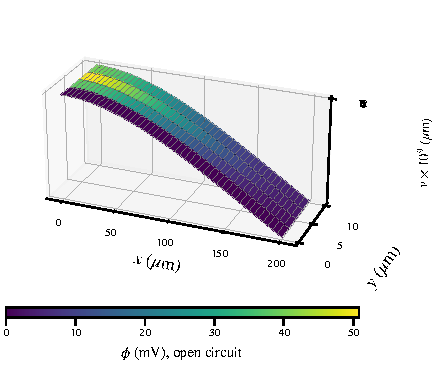
\includegraphics[width=\textwidth]{FB2_modes.pdf}
\caption{Open-circuit bending mode and its potential field. The three-dimensional surface is the computed transverse displacement in nanometers, colored by the solved electric potential; the inset shows labeled potential contours on the strip coordinates, with contour labels in millivolts. Both views use the same finite-element solution and the same assumed inputs as Fig.~\ref{fig:fields}.}
\label{fig:modes}
\end{figure}

%% generated table -- do not edit (see AUTHOR_TODO.md)
\begin{table}[!htbp]
\centering
\small
\caption{Thickness sweep behind Fig.~\ref{fig:thickness}. First frequency,
flexoelectric bending coupling and extensional coupling of the poled strip. The
bending column carries $\mu=10^{-6}$\,\si{\coulomb\per\metre}, the extensional
column $\mu=0$, and both are converged to the tolerance of
\ref{app:verification}.}
\label{tab:thickness}
\begin{tabular}{@{}r r r r@{}}
\toprule
$h$ (\si{\micro\metre}) & $f_1$ (kHz) & $k^2_{\rm flexo}$ & $k^2_{\rm piezo}$ \\
\midrule
10 & 210.4 & 1.744e-04 & 0.55814 \\
7 & 148.7 & 3.510e-04 & 0.55831 \\
5 & 108.0 & 6.587e-04 & 0.55843 \\
3.5 & 78.2 & 1.218e-03 & 0.55851 \\
2.7 & 62.9 & 1.808e-03 & 0.55855 \\
2 & 50.2 & 2.642e-03 & 0.55858 \\
1.4 & 40.3 & 3.608e-03 & 0.55860 \\
1 & 34.7 & 4.174e-03 & 0.55861 \\
\bottomrule
\end{tabular}
\end{table}


\subsubsection{The piezoelectric coupling is thickness independent}

Panel~(b) of Fig.~\ref{fig:thickness} is the counterpart of panel~(a). The
quasi-static extensional coupling takes the values $0.55814$, $0.55843$,
$0.55858$ and $0.55861$ at $10$, $5$, $2$ and \SI{1}{\micro\meter}, that is it
changes by $0.09\,\%$ between \SI{10}{\micro\meter} and \SI{1}{\micro\meter},
against the constitutive closed form $0.5608$ for the same material and the
same plane-stress kinematics. The piezoelectric effect is a bulk effect, so a
thinner strip is electromechanically neither better nor worse, whereas the
flexoelectric effect is a gradient effect and improves by a factor $24$ over
the same range. A device can therefore be thinned for the flexoelectric
response without a penalty in the piezoelectric one, and the crossover
thickness is a property of the window and of $\mu$, not of the piezoelectric
constants.

\subsubsection{What the piezoelectric terms do on the bending device}

The bending configuration is poled along $y$ with electrodes on the long faces,
and the crystal carries $e_{31}$ and $e_{33}$ as well, so the two effects can
be separated inside one run. With $\mu=0$ the piezoelectric coupling of that
mode is $1.0\times10^{-10}$ at every thickness, because the piezoelectric charge
$e_{31}\varepsilon_{xx}+e_{33}\varepsilon_{yy}$ is odd in $y-h/2$ and its
integral over a face electrode vanishes, so the arrangement carries no net
piezoelectric charge. With $e=0$ the flexoelectric coupling runs from
$1.76\times10^{-4}$ to $5.5\times10^{-3}$, a factor $31$, while the full crystal
gives the $24$ reported above: the piezoelectric terms shift the flexoelectric
coupling by up to $24\,\%$ at the thinnest strip, through the elastic stiffness
of the same mode rather than through a charge they contribute. The number
quoted in the abstract and in Fig.~\ref{fig:thickness} is the full-crystal one.

\subsubsection{Numerical reproducibility of the thinnest point}

The $h=\SI{1}{\micro\meter}$ point is the least reproducible number in the
paper. Its $k^2$ is a difference of two nearly equal eigenvalues of a pencil
whose condition number is $\sim10^{12}$ at that thickness, so the number
carries the accuracy of the eigensolver: four mathematically equivalent
eigensolver paths and four numeric stacks agree on $4.2\times10^{-3}$ and on
the factor $24$ to within $0.5\,\%$. The spread quoted is the range over the
midpoint of those equivalent results, and at $h=\SI{10}{\micro\meter}$ it is
at most $10^{-4}\,\%$. Values are quoted to two significant digits. Hence
thinning the strip multiplies the flexoelectric bending coupling by $24$ while
leaving the piezoelectric extensional coupling unchanged to $0.09\,\%$, which
is the size effect that this model was built to separate from the material
property. The estimate \eqref{eq:xflexo} is the $h^{-2}$ guide drawn in
panel~(a), and the inverse route \eqref{eq:muV} of Sec.~\ref{sec:calib_a_mu}
is the one that would measure $\mu$ rather than assume it.

\FloatBarrier
\subsection{The design map}
\label{sec:designmap}

Figure~\ref{fig:designmap} shows the two couplings of the third question on one
grid, which a designer needs because they are not comparable in size and a device
has to be designed against both at once. They depend on different variables: the flexoelectric bending coupling on the thickness and on the
window, the piezoelectric extensional coupling on neither. Figure~\ref{fig:designmap}
resolves them over the same two parameters. Panel~(a) is the flexoelectric
bending coupling on a grid of eight thicknesses and eight window
half-thicknesses, computed with the mode-based measure \eqref{eq:k2mode} and
the same $48\times4$ mesh as Fig.~\ref{fig:thickness}(a); panel~(b) is the
ratio of that bending coupling to the mode-free extensional coupling
\eqref{eq:kstatic} of the same strip. Both panels carry the line $a_2=h$, along which
the window is as thick as the strip, and the map stops at $a_2/L=0.2$, the
operating range assumed in Sec.~\ref{sec:limit_window}.

The map has three features worth naming. First, the coupling is controlled by
the ratio $a_2/h$ rather than by the thickness alone. At
$h=\SI{10}{\micro\meter}$ shrinking the window half-thickness from $1$ to
$0.25\,\mu$m changes the coupling from $1.7\times10^{-4}$ to
$1.6\times10^{-4}$, a change of $5.5\,\%$, because the window is far thinner
than the strip in both cases; at $h=\SI{1}{\micro\meter}$ the same change of
window takes the coupling from $4.2\times10^{-3}$ to $1.0\times10^{-2}$, a
factor $2.5$. Second, the window is the stronger lever of the two once it is
comparable to the strip: over the whole map the coupling spans
$3.6\times10^{-6}$ to $1.0\times10^{-2}$, of which the thickness alone
accounts for the factor $24$ of Fig.~\ref{fig:thickness}(a). Third, the two
couplings never become comparable at these parameters: the ratio in panel~(b)
spans $6.5\times10^{-6}$ to $1.9\times10^{-2}$, and it reaches $0.1\,\%$ only
below $h=5.5\,\mu$m for the window of the paper, $a_2=\SI{1}{\micro\meter}$.
The map is quoted to two significant digits because its thin-strip entries are
differences of nearly equal eigenvalues and move in the third digit across
numeric stacks.
The design rule that follows is that the window should be chosen for the
gradient one wants to resolve and the thickness for the size effect one wants
to exploit; and that a device in which the two couplings are meant to compete
needs a window thinner than the strip and a flexoelectric coefficient two
orders of magnitude larger than the value assumed here. The map therefore distinguishes the effect of thickness from the suppression
caused by the gradient stiffness.

\begin{figure}[!htbp]
\centering
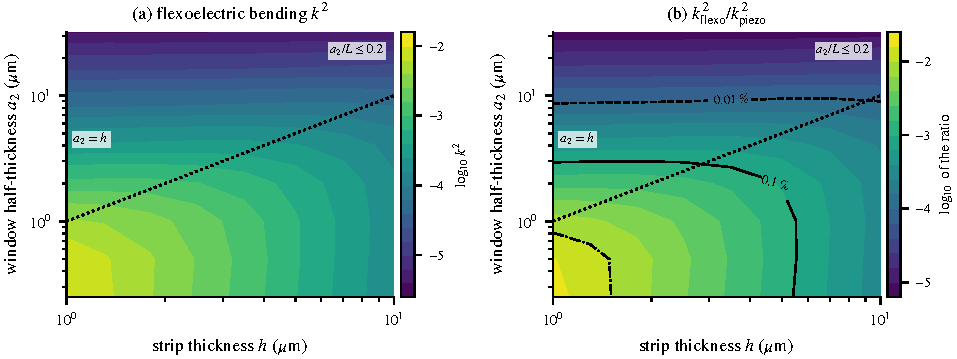
\includegraphics[width=\textwidth]{F11_designmap.pdf}
\caption{Variations of (a) the flexoelectric bending coupling and of (b) its ratio to the piezoelectric extensional coupling over strip thickness and window half-thickness, for $L=\SI{200}{\micro\meter}$ and $a_1=\SI{3}{\micro\meter}$, with the $0.01\,\%$ and $0.1\,\%$ contours. The dotted line is $a_2=h$ and the map ends at the assumed $a_2/L=0.2$.}
\label{fig:designmap}
\end{figure}

\FloatBarrier
\subsection{Transient response and the memory model}
\label{sec:transient}

Figure~\ref{fig:ringdown} shows the ring-down of the extensional mode in the
time domain, which is the memory question of Sec.~\ref{sec:memorystudy} seen as
a device records it, because a damping ratio is a frequency-domain summary and a
sensor is read in time. The strip starts from a tip displacement of
\SI{10}{\nano\meter} and is followed for eight Caputo orders between
$\alpha=1$ and $0.4$ at fixed $\tau=\SI{3}{\nano\second}$
($\omega\tau=0.13$): the tip displacement in panel~(a) and the open-circuit
voltage in panel~(b). The initial voltage, \SI{139}{\volt}, is set by the mode
shape and the electrode configuration and is independent of $\alpha$, as it
must be, since the memory term vanishes at $t=0^{+}$; the decay rate, by
contrast, depends on $\alpha$. The $\alpha=1$ curve is the exponential decay of
the classical Kelvin--Voigt element, while the fractional curves are not
exponential, and it is that difference which the damping map of
Fig.~\ref{fig:damping}(b) quantifies. Over the eight orders plotted, the
decrement of the tip displacement over the first two peaks, converted with
\eqref{eq:zeta}, runs from $0.063$ at $\alpha=1$ to a maximum of $0.104$ at
$\alpha=0.6$ and back to $0.085$ at $\alpha=0.4$
(Table~\ref{tab:ringdown}). For $\alpha<1$ it is a first-period decrement and
not a damping ratio, because those records are not exponential; a design that
takes the integer-order early decay as representative is in error by $64\,\%$
at $\alpha=0.6$, and the sign of the error cannot be guessed from $\alpha$
alone. Hence a recorded ring-down identifies the pair $(\alpha,\tau)$ only if
the order is known from an independent measurement, which is the route taken in
Sec.~\ref{sec:calibration}. The march is the one of \eqref{eq:newmark} with the
L1 history, and the decrement is converted with \eqref{eq:zeta}.

\begin{figure}[!htbp]
\centering
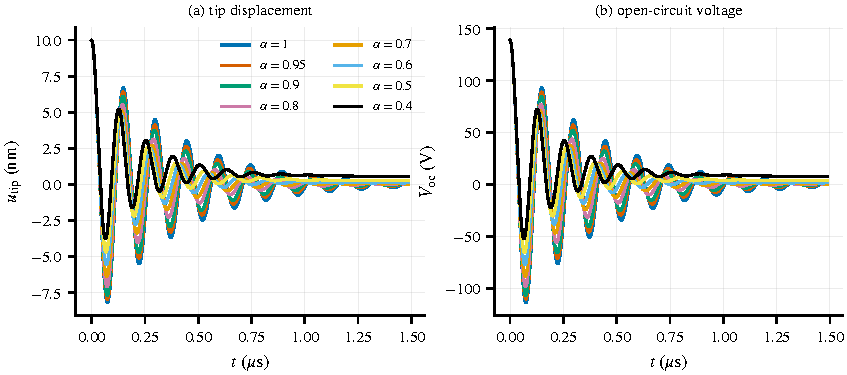
\includegraphics[width=\textwidth]{F9_ringdown.pdf}
\caption{Variations of (a) the tip displacement and (b) the open-circuit voltage of the extensional mode at \SI{6.727}{MHz} for eight Caputo orders, with modal memory on $K_{\rm eff}$, eight modes, $\tau=\SI{3}{\nano\second}$ ($\omega\tau=0.13$), an initial tip displacement of \SI{10}{\nano\meter} and $4000$ L1 steps over ten periods. Only the $\alpha=1$ decay is exponential.}
\label{fig:ringdown}
\end{figure}

\FloatBarrier
\subsection{Application: a \SI{200}{\micro\meter} by \SI{10}{\micro\meter}
strip in open-circuit sensing}
\label{sec:application}

The worked case is a \SI{200}{\micro\meter} long, \SI{10}{\micro\meter} thick
$\mathrm{BaTiO_3}$ strip clamped on one short edge, poled along its length and
electroded on the two ends: the strain in the active region is extensional, so
the piezoelectric coupling dominates and the flexoelectric term is a
size-dependent correction. Table~\ref{tab:application} collects the four
polarization/kinematics combinations of that strip, each solved from the
condensed system \eqref{eq:saddle} with the electrode charge
\eqref{eq:electrode}, and each quoted using the mode-based coupling \eqref{eq:k2mode}. The lowest-frequency mode of the
extensional configuration is at \SI{147.73}{kHz}, above the clamped-free value
of a beam of the same length because the gradient terms stiffen the member,
while the strongly coupled extensional mode sits at \SI{6725.8}{kHz}.

\begin{table}[!htbp]
\centering
\small
\caption{The coupling of the strongest mode, its frequency and the
open-circuit voltage at \SI{10}{\nano\meter} of tip motion, for a
\SI{200}{\micro\meter}$\times$\SI{10}{\micro\meter} strip in four polarization
and kinematics combinations. The two plane-stress rows are the configurations
of Fig.~\ref{fig:geometry}, and the couplings of the four rows are not
additive.}
\label{tab:application}
% table generated from the archived results
\begin{tabular}{@{}llcccc@{}}
\toprule
poling & kinematics & mode & $f$ (kHz) & $k^2$ & $V$ at \SI{10}{\nano\metre} (V) \\
\midrule
y & plane strain & bending (4) & 6721.8 & 0.1749 & 3.48 \\
y & plane stress & bending (4) & 6361.0 & 0.1141 & 2.41 \\
x & plane strain & extensional (5) & 7161.0 & 0.4024 & 141.45 \\
x & plane stress & extensional (5) & 6725.8 & 0.4580 & 138.99 \\
\bottomrule
\end{tabular}

\end{table}

Three consequences follow.

\begin{enumerate}
\item \textbf{The electrode arrangement dominates.} Poling along the length
  gives $k^2=0.4580$ and \SI{138.99}{\volt} at \SI{10}{\nano\meter} of motion;
  the bending configuration gives $0.1141$ and \SI{2.41}{\volt} -- a factor
  $58$ in voltage at equal amplitude and a factor four in $k^2$. The handicap
  belongs to the arrangement, not to $e_{31}$: a symmetric strip bent between
  full through-thickness electrodes collects almost no net charge.
\item \textbf{The quasi-static coupling is $0.5581$} and thickness independent
  (Sec.~\ref{sec:thickness}): the number to quote far below the first
  resonance, and the one that survives thinning.
\item \textbf{The damping is set by $(\alpha,\tau)$ and by the memory matrix},
  not by a material constant: at $\omega\tau=0.3$ and $\alpha=1$,
  $\zeta_{\rm eff}=0.15003$ on $K_{\rm eff}$ against $0.0675$ on $K_{uu}$, a
  ratio of $0.450$. A damping number quoted without $\alpha$, $\tau$ and the
  memory matrix is under-specified.
\end{enumerate}

These numbers are the output of the model, and each of them rests on an input
that no constitutive table supplies; Sec.~\ref{sec:calibration} identifies those
inputs one at a time and states the ranges over which the numbers hold.

\FloatBarrier
